\documentclass{beamer}

\usetheme{Warsaw}
\usepackage{hyperref}
\usepackage{graphicx}


\title{Retrofit Learning Management System Using SCORM}

\author{Mingkun Yang \\
\texttt{minyan09@student.hh.se}}

\institute{
Halmstad University\\
}
\date{}

\AtBeginSection[]
{
\begin{frame}<beamer>{Outline}
	\tableofcontents[currentsection]
\end{frame}
}

\begin{document}

\begin{frame}
	\titlepage
\end{frame}

\begin{frame}{Outline}
	\tableofcontents[pausesections]
\end{frame}

\section{Introduction}
\begin{frame}{Background}
	\begin{itemize}
		\item
			Learning Management System(LMS)
			\pause
		\item
			Sharable Content Object Reference Model(SCORM)
			\pause
		\item
			Sharable Content Object(SCO)
	\end{itemize}
\end{frame}
\begin{frame}{Package VS SCO}
	C Programming Language
	\begin{itemize}
		\item
			Syntax
		\item
			Pointer
		\item
			Structure
		\item
			\ldots
	\end{itemize}
\end{frame}
\begin{frame}{Objectives}
	\begin{itemize}
		\item
			Importing whole package
		\item
			Importing single SCOs
		\item
			Exporting whole package
		\item
			Launching single SCOs
	\end{itemize}
\end{frame}

\section{Method}
\begin{frame}{Framework}
	ASP.NET MVC framework
	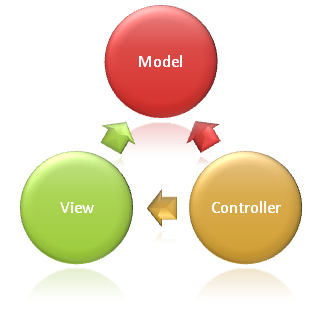
\includegraphics[width=100mm, height=60mm]{mvc_framework.png}
\end{frame}
\begin{frame}{Database}
	Database
	\hspace*{-5mm}
	\includegraphics[width=120mm, height=60mm]{database_layout.png}
\end{frame}

\section{Result}
\begin{frame}{User interface of LMS for importing}
	\hspace*{-5mm}
	\includegraphics[width=120mm, height=60mm]{importing.png}
\end{frame}
\begin{frame}{Result of importing whole package}
	\hspace*{-5mm}
	\includegraphics[width=120mm, height=60mm]{result_import_whole_package.png}
\end{frame}
\begin{frame}{Result of importing single SCOs}
	\hspace*{-5mm}
	
\includegraphics[width=120mm, height=60mm]{result_import_single_scos.png}
\end{frame}
\begin{frame}{Result of previewing single SCOs}
	\hspace*{-5mm}
	\includegraphics[width=120mm, height=60mm]{result_presentation_sco.png}
\end{frame}

\section{Conclusion}
\begin{frame}{Separation of concerns}
	\begin{itemize}
		\item
			\pause
			MVC architect
			\pause
		\item
			Modularity Programming
			\pause
		\item
			\LaTeX
			\pause
	\end{itemize}
\end{frame}
\begin{frame}{To be continue}
	\begin{itemize}
		\item
			Communication between SCO and LMS
			\pause
		\item
			Sequencing between SCOs
			\pause
	\end{itemize}
\end{frame}
\end{document}
